
\subsection{Iteración 3}


En esta última iteración para esta entrega se busca conocer la respuesta de varios usuarios ante los escenarios desarrollados. Parte de esta iteración se ha realizado en paralelo a la anterior, durante el desarrollo de los escenarios. Esto ha permitido realizar un trabajo más efectivo desde una fase temprana de la entrega. Esta vez solo se ha podido contar con una persona para que ofrezca su opinión y críticas sobre el trabajo desarrollado. 

Esta persona tiene entre 20 y 30 años y tiene un amplio conocimiento tecnológico pero una experiencia limitada en realidad virtual. Para la realización de la prueba se ha colocado al usuario en el centro del escenario y se le ha dado libertad de desplazamiento por todo el escenario mientras se iba conversando para obtener información útil. 

De esta prueba han surgido varios pequeños cambios que ya han sido realizados en el proyecto, la mayoría relacionados con la posición de ciertos objetos, como la pantalla que estaba demasiado alta. Pero sin duda, el factor más importante para tener en cuenta es la escala y tamaño de los objetos del mundo virtual. Es necesario que la escala del entorno sea lo más parecida a la realidad, ya que de otra forma crea situaciones incómodas como: mesas demasiado altas o bajas, modelos de personas que parecen ser gigantes, o un espacio demasiado grande y vacío.

Finalmente, tras tomar en consideración toda esta información, se ha ido adaptando el escenario hasta su forma final, que se puede ver en la figura \ref{fig:E3_escenarioCompleto}.


\begin{figure}
  \centering
    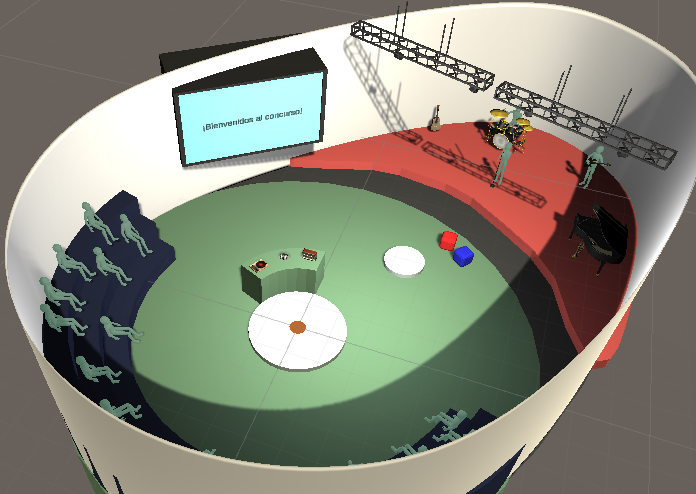
\includegraphics[width=0.5\textwidth]{04.Desarrollo/03.Entrega3/03.Iteracion3_3/00.Figuras/01.unity_6.png}
    \caption{Montaje final del escenario para la entrega 3.}
    \label{fig:E3_escenarioCompleto}
\end{figure}






